\documentclass{beamer}
\usepackage[latin1]{inputenc}

\usetheme{Madrid}
\usecolortheme{default}
\usepackage{amsmath}
\usepackage{amssymb,amsfonts,amsthm}
\usepackage{txfonts}
\usepackage{tkz-euclide}
\usepackage{listings}
\usepackage{adjustbox}
\usepackage{array}
\usepackage{tabularx}
\usepackage{gvv}
\usepackage{lmodern}
\usepackage{circuitikz}
\usepackage{tikz}
\usepackage{graphicx}
\usepackage{gensymb}
\usepackage{physics}

\setbeamertemplate{page number in head/foot}[totalframenumber]

\usepackage{tcolorbox}
\tcbuselibrary{minted,breakable,xparse,skins}



\definecolor{bg}{gray}{0.95}
\DeclareTCBListing{mintedbox}{O{}m!O{}}{%
  breakable=true,
  listing engine=minted,
  listing only,
  minted language=#2,
  minted style=default,
  minted options={%
    linenos,
    gobble=0,
    breaklines=true,
    breakafter=,,
    fontsize=\small,
    numbersep=8pt,
    #1},
  boxsep=0pt,
  left skip=0pt,
  right skip=0pt,
  left=25pt,
  right=0pt,
  top=3pt,
  bottom=3pt,
  arc=5pt,
  leftrule=0pt,
  rightrule=0pt,
  bottomrule=2pt,
  toprule=2pt,
  colback=bg,
  colframe=orange!70,
  enhanced,
  overlay={%
    \begin{tcbclipinterior}
    \fill[orange!20!white] (frame.south west) rectangle ([xshift=20pt]frame.north west);
    \end{tcbclipinterior}},
  #3,
}
\lstset{
    language=C,
    basicstyle=\ttfamily\small,
    keywordstyle=\color{blue},
    stringstyle=\color{orange},
    commentstyle=\color{green!60!black},
    numbers=left,
    numberstyle=\tiny\color{gray},
    breaklines=true,
    showstringspaces=false,
}
\title{7.4.32}
\date{4th october, 2025}
\author{Vishwambhar - EE25BTECH11025}

\begin{document}

\frame{\titlepage}
\begin{frame}{Question}
$ABCD$ is a square of side length 2 units. $C_1$ is the circle touching all the sides of the square $ABCD$ and $C_2$ is the circumcircle of square $ABCD$. $L$ is a fixed line in same plane and $\vec{R}$ is a fixed point.\\
\begin{enumerate}
    \item If $\vec{P}$ is any point of $C_1$ and $\vec{Q}$ is another point on $C_2$, then $\frac{PA^2+PB^2+PC^2+PD^2}{QA^2+QB^2+QC^2+QD^2}$
    \begin{enumerate}
        \item 0.75
        \item 1.25
        \item 1
        \item 0.5
    \end{enumerate}
    \end{enumerate}
    \end{frame}
    \begin{frame}
    \begin{enumerate}
    \item If a circle is such that it touches the line $L$ and the circle $C_1$ externally, such that both the circles are on the same side of the line, then locus of centre of the circle
    \begin{enumerate}
        \item ellipse
        \item hyperbola
        \item parabola
        \item circle
    \end{enumerate}
    \item A $L'$ through $\vec{A}$ is drawn parallel to $BD$. Point $S$ moves such that its distances from the line $BD$ and the vertex $\vec{A}$ are equal. If locus of $S$ cuts $L'$ at $T_2$ and $T_3$ and $AC$ at $T_1$, then area of $\triangle T_1T_2T_3$ is
    \begin{enumerate}
        \item 1/2 sq.units
        \item 2/3 sq.units
        \item 1 sq.units
        \item 2 sq.units
    \end{enumerate}
\end{enumerate}
\end{frame}
\begin{frame}{Let}
Let:\\
The centre of incircle and circumcircle be $\vec{O}$.\\
The radius of incircle be $r_1$ and that of circumcircle be $r_2$.\\
Given:
\begin{align}
    r_1 = 1\\
    r_2 = \sqrt{2}
\end{align}
\end{frame}

\begin{frame}{1st question}
Let $\vec{P}$ be any point on incircle and $\vec{Q}$ be any point on circumcircle.\\
$\vec{X}\epsilon \cbrak{\vec{A,B,C,D}}$
\begin{align}
    \norm{\vec{X}-\vec{P}}^2 = \norm{\vec{X}}^2 + \norm{\vec{P}}^2 - 2\vec{P}.\vec{X}\\
\end{align}
Summation over all $\vec{X}|\vec{X}\epsilon \cbrak{\vec{A,B,C,D}}$:
\begin{align}
    \sum \norm{\vec{X}-\vec{P}}^2 = \sum \norm{\vec{X}}^2 + 4.\norm{\vec{P}}^2 -2\vec{P}\sum \vec{X}\\
\end{align}
\end{frame}

\begin{frame}{1st question}
For, $\vec{P}$ = $\vec{P}$
\begin{align}
    \sum \norm{\vec{X}-\vec{P}}^2 = \sum \norm{\vec{X}}^2 + 4.\norm{\vec{P}}^2 -2\vec{P}\sum \vec{X}\\
    4\brak{1^2+1^2} + 4\brak{1}-2\vec{P}\brak{\myvec{1\\1}+\myvec{1\\-1}+\myvec{-1\\1}+\myvec{-1\\-1}}\\
    \therefore \norm{\vec{A}-\vec{P}}^2+\norm{\vec{B}-\vec{P}}^2+\norm{\vec{C}-\vec{P}}^2+\norm{\vec{D}-\vec{P}}^2 = 12
\end{align}
\end{frame}

\begin{frame}{1st question}
For, $\vec{P}$ = $\vec{Q}$
\begin{align}
    \sum \norm{\vec{X}-\vec{Q}}^2 = \sum \norm{\vec{X}}^2 + 4.\norm{\vec{Q}}^2 -2\vec{Q}\sum \vec{X}\\
    4\brak{1^2+1^2} + 4\brak{2}-2\vec{Q}\brak{\myvec{1\\1}+\myvec{1\\-1}+\myvec{-1\\1}+\myvec{-1\\-1}}\\
    \therefore \norm{\vec{A}-\vec{Q}}^2+\norm{\vec{B}-\vec{Q}}^2+|\norm{\vec{C}-\vec{Q}}^2+norm{\vec{D}-\vec{Q}}^2 = 12
\end{align}
\end{frame}

\begin{frame}{1st question}
    conclusion:
\begin{align}
    \frac{12}{16}=0.75
\end{align}
Hence, option(a) is correct.
\end{frame}

\begin{frame}{2nd question}
    Let the radius of the moving circle be $r$, the centre of the circle be $\vec{X}$ and the line equation be $\vec{\hat{n}}^\top\vec{X}=c$,
\end{frame}

\begin{frame}{2nd question}
    \begin{align}
    |\vec{\hat{n}}^\top\vec{X}-c|=r\\
    ||\vec{X}||=r+1\\
    ||\vec{X}||=|\vec{\hat{n}}\vec{X}-\brak{c-1}|\\
    ||\vec{X}||^2=|\vec{\hat{n}}\vec{X}-\brak{c-1}|^2\\
    \vec{X}^\top\vec{X}=\brak{\vec{\hat{n}^\top\vec{X}}}^2+\brak{c-1}^2-2\vec{\hat{n}}^\top\vec{X}\brak{c-1}\\
    \vec{X}^\top\vec{X}-\brak{\vec{\hat{n}}\vec{X}}^2+2\vec{\hat{n}^\top\vec{X}}\brak{c-1}-\brak{c-1}^2\\
    \vec{X}^\top\brak{I-\vec{\hat{n}}\vec{\hat{n}}^\top}\vec{X}+2\brak{c-1}\vec{\hat{n}^\top\vec{X}}-\brak{c-1}^2
\end{align}
\end{frame}

\begin{frame}{2nd question}
Equation (20) is the equation of parabola.\\
Hence, correct option is (c).
\end{frame}

\begin{frame}{3rd question}
    Let the point moving point be $S$ and the line equation be $\vec{n}^\top\vec{S}=0$.
\begin{align}
    \frac{|\vec{n}^\top\vec{S}|}{||\vec{n}||}=||\vec{S}-\vec{A}||\\
    \frac{|\vec{n}^\top\vec{S}|^2}{||\vec{n}||^2}=||\vec{S}-\vec{A}||^2\\
    \frac{|\vec{S}^\top\vec{n}\vec{n}^\top\vec{S}|}{||\vec{n}||}=\brak{\vec{S}-\vec{A}}^\top\brak{\vec{S}-\vec{A}}\\
    \vec{S}^\top\brak{I-\vec{\hat{n}}\vec{\hat{n}}^\top}\vec{S}-2\vec{A}^\top\vec{S}+\vec{A}^\top\vec{A}=0
\end{align}
\end{frame}

\begin{frame}{3rd question}
    Equation 24 is the locus of the moving point.\\
Let:
\begin{align}
    \vec{A}=\myvec{1\\1};\vec{B}=\myvec{-1\\1}\\
    \vec{C}=\myvec{-1\\-1};\vec{D}=\myvec{1\\-1}
\end{align}
$\vec{m_1}$ be the direction vector of line AC, $\vec{m_2}$ be the direction vector of line $L'$.
\begin{align}
    \vec{m_1} = \myvec{-2\\-2}=\myvec{1\\1}\\
    \vec{m_2} = \myvec{2\\-2}
\end{align}
\end{frame}

\begin{frame}{3rd question}
    The equation of line $L'$ 
\begin{align} \vec{S}=\vec{A}+t\vec{m_2}\end{align}
The equation of the line AC
\begin{align}
\vec{S}=\lambda \vec{m_1}
\end{align}
Substituting equation (30) in (24) we get $\lambda=\frac{1}{2}$:
\begin{align}
    \vec{T_1}=\frac{1}{2}\myvec{1\\1}
\end{align}
\end{frame}

\begin{frame}{3rd question}
    Substituting (29) in (24) we get $t=\frac{-1}{2},\frac{1}{2}$
\begin{align}
    \vec{T_2}=\myvec{0\\2}\\
    \vec{T_3}=\myvec{2\\0}
\end{align}
Now, finding area of the triangle:
\begin{align}
    \triangle T_1T_2T_3=\frac{1}{2}\norm{\myvec{\vec{T_2}-\vec{T_1}&\vec{T_3}-\vec{T_2}}}\\
    \triangle T_1T_2T_3 = 1
\end{align}
Option (c) is correct.
\end{frame}
\begin{frame}[fragile]
    \frametitle{C Code}
    \begin{lstlisting}
#include <stdio.h>
#include <math.h>
void get_results(double *out_data) {
    double side = 2.0;
    double r1 = side / 2.0;          
    double r2 = side / sqrt(2.0);   
    double ratio = (r1 * r1 + r1 * r1 + r1 * r1 + r1 * r1) /
                   (r2 * r2 + r2 * r2 + r2 * r2 + r2 * r2);
    double k = 2.0;
    double focus_x = 0.0;
    double focus_y = k + r1;
    double directrix_y = k - r1;
    double area = 2.0 / 3.0;
    \end{lstlisting}
\end{frame}

\begin{frame}[fragile]
    \frametitle{C code}
    \begin{lstlisting}
    double a = 1;
    double b = -1;
    out_data[0] = ratio;
    out_data[1] = focus_x;
    out_data[2] = focus_y;
    out_data[3] = directrix_y;
    out_data[4] = area;
    out_data[5] = a; //Ax
    out_data[6] = a; //Ay
    out_data[7] = b; //Bx
    out_data[8] = a; //By
    out_data[9] = b; //Cx
    out_data[10] = b; //Cy
    out_data[11] = a; //Dx
    out_data[12] = b; //Dy
    out_data[13] = 0.5; //T1x
    out_data[14] = 0.5; //T1y;
    out_data[15] = 0; //T2x;
    out_data[16] = 2; //T2y
    out_data[17] = 2; //T3x
    out_data[18] = 0; //T3y 
}
    \end{lstlisting}
\end{frame}

\begin{frame}[fragile]
    \frametitle{call.py}
    \begin{lstlisting}
import ctypes as ct
import numpy as np
def get_results():
    lib = ct.CDLL("./problem.so")
    lib.get_results.argtypes = [ct.POINTER(ct.c_double)]
    data_type = ct.c_double * 19
    data = data_type()
    lib.get_results(data)
    arr = np.array(list(data))
    ratio, focus_x, focus_y, directrix_y, area, Ax, Ay, Bx, By, Cx, Cy, Dx, Dy, T1x, T1y, T2x, T2y, T3x, T3y= arr
    return ratio, np.array([focus_x, focus_y]), directrix_y, area, Ax, Ay, Bx, By, Cx, Cy, Dx, Dy, T1x, T1y, T2x, T2y, T3x, T3y
    \end{lstlisting}
\end{frame}

\begin{frame}[fragile]
    \frametitle{plot1.py}
    \begin{lstlisting}
import numpy as np
import matplotlib.pyplot as plt
from call import get_results
ratio, focus, directrix_y, area, Ax, Ay, Bx, By, Cx, Cy, Dx, Dy, T1x, T1y, T2x, T2y, T3x, T3y = get_results()
theta = np.linspace(0, 2*np.pi, 200)
A = ([Ax, Bx, Cx, Dx, Ax, Bx])
B = ([Ay, By, Cy, Dy, Ay, By])
plt.plot(A, B, color='black')
plt.text(Ax+0.1, Ay+0.1, "A", fontsize = 10, color = 'black')
plt.text(Bx+0.1, By+0.1, "B", fontsize = 10, color = 'black')
    \end{lstlisting}
\end{frame}

\begin{frame}[fragile]
    \frametitle{plot1.py}
    \begin{lstlisting}
plt.text(Cx+0.1, Cy+0.1, "C", fontsize = 10, color = 'black')
plt.text(Dx+0.1, Dy+0.1, "D", fontsize = 10, color = 'black')
plt.plot(np.cos(theta), np.sin(theta), label="Inner Circle C1")
plt.plot(np.sqrt(2)*np.cos(theta), np.sqrt(2)*np.sin(theta), label="Outer Circle C2")
plt.axis("equal")
plt.grid(True)
plt.savefig("../figs/plot1.png")
plt.show()
    \end{lstlisting}
\end{frame}

\begin{frame}[fragile]
    \frametitle{plot2.py}
    \begin{lstlisting}
import numpy as np
import matplotlib.pyplot as plt
from call import get_results
ratio, focus, directrix_y, area, Ax, Ay, Bx, By, Cx, Cy, Dx, Dy, T1x, T1y, T2x, T2y, T3x, T3y = get_results()
A = ([Ax, Bx, Cx, Dx, Ax, Bx])
B = ([Ay, By, Cy, Dy, Ay, By])
x = np.linspace(-5, 5, 300)
p = focus[1] - directrix_y
y = (x**2) / (4*p)
plt.plot(x, y, label="Locus (Parabola)")
plt.axhline(directrix_y, color='r', linestyle='--', label='Directrix')
plt.plot(focus[0], focus[1], 'go')
    \end{lstlisting}
\end{frame}

\begin{frame}[fragile]
    \frametitle{plot2.py}
    \begin{lstlisting}
plt.text(Ax+0.1, Ay+0.1, "A", fontsize = 10, color = 'black')
plt.text(Bx+0.1, By+0.1, "B", fontsize = 10, color = 'black')
plt.text(Cx+0.1, Cy+0.1, "C", fontsize = 10, color = 'black')
plt.text(Dx+0.1, Dy+0.1, "D", fontsize = 10, color = 'black')
plt.text(focus[0]+0.1, focus[1]+0.1, 'focus', fontsize = 10, color = 'black')
plt.axis("equal")
plt.grid(True)
plt.savefig("../figs/plot2.png")
plt.show()
    \end{lstlisting}
\end{frame}

\begin{frame}[fragile]
    \frametitle{plot3.py}
    \begin{lstlisting}
import numpy as np
import matplotlib.pyplot as plt
from call import get_results
ratio, focus, directrix_y, area, Ax, Ay, Bx, By, Cx, Cy, Dx, Dy, T1x, T1y, T2x, T2y, T3x, T3y = get_results()
A = ([Ax, Bx, Cx, Dx, Ax, Bx])
B = ([Ay, By, Cy, Dy, Ay, By])
C = ([T1x, T2x, T3x, T1x, T2x])
D = ([T1y, T2y, T3y, T1y, T2y])
triangle = np.array([[0,0], [2,0], [1, np.sqrt(3)/2]])
plt.plot(A, B, color='black')
    \end{lstlisting}
\end{frame}

\begin{frame}[fragile]
    \frametitle{plot3.py}
    \begin{lstlisting}
plt.text(Ax+0.1, Ay+0.1, "A", fontsize = 10, color = 'black')
plt.text(Bx+0.1, By+0.1, "B", fontsize = 10, color = 'black')
plt.text(Cx+0.1, Cy+0.1, "C", fontsize = 10, color = 'black')
plt.text(Dx+0.1, Dy+0.1, "D", fontsize = 10, color = 'black')
plt.plot(C, D, color='black') 
plt.text(T1x+0.1, T1y+0.1, "T1", fontsize = 10, color = 'black')
plt.text(T2x+0.1, T2y+0.1, "T2", fontsize = 10, color = 'black')
plt.text(T3x+0.1, T3y+0.1, "T3", fontsize = 10, color = 'black')
plt.axis("equal")
plt.grid(True)
plt.savefig("../figs/plot3.png")
plt.show()
    \end{lstlisting}
\end{frame}

\begin{frame}{Plot}
    \begin{figure}
        \centering
        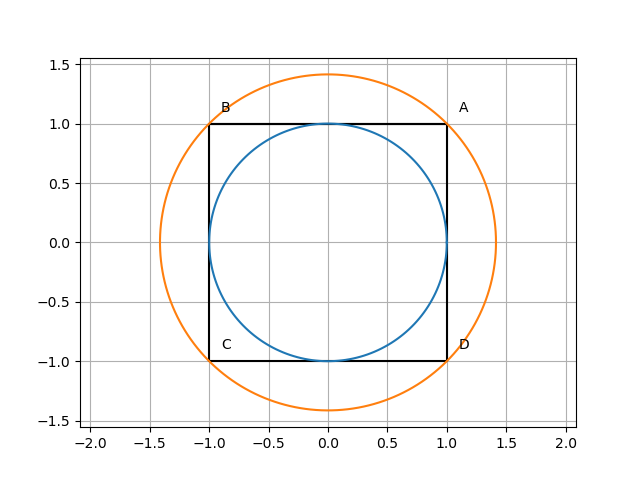
\includegraphics[width=0.5\columnwidth]{../figs/plot1.png}
        \caption{Plot of the given square and circles}
        \label{fig:fig}
    \end{figure}
\end{frame}

\begin{frame}{Plot}
    \begin{figure}
        \centering
        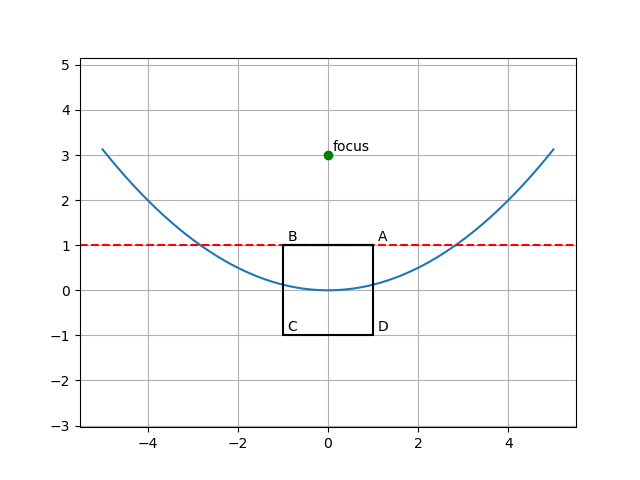
\includegraphics[width=0.5\columnwidth]{../figs/plot2.png}
        \caption{Plot of the given circles, square and locus of the point }
        \label{fig:fig}
    \end{figure}
\end{frame}

\begin{frame}{Plot}
    \begin{figure}
        \centering
        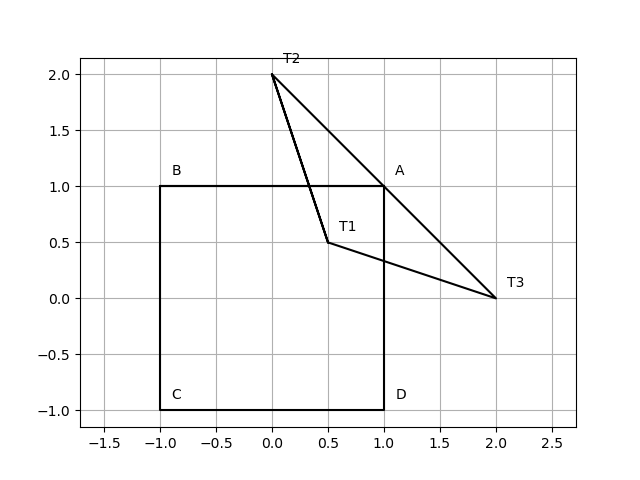
\includegraphics[width=0.5\columnwidth]{../figs/plot3.png}
        \caption{Plot of the given circles, square and locus of the point }
        \label{fig:fig}
    \end{figure}
\end{frame}

\end{document}